% Options for packages loaded elsewhere
\PassOptionsToPackage{unicode}{hyperref}
\PassOptionsToPackage{hyphens}{url}
\PassOptionsToPackage{dvipsnames,svgnames,x11names}{xcolor}
%
\documentclass[
  letterpaper,
  DIV=11,
  numbers=noendperiod]{scrartcl}

\usepackage{amsmath,amssymb}
\usepackage{iftex}
\ifPDFTeX
  \usepackage[T1]{fontenc}
  \usepackage[utf8]{inputenc}
  \usepackage{textcomp} % provide euro and other symbols
\else % if luatex or xetex
  \usepackage{unicode-math}
  \defaultfontfeatures{Scale=MatchLowercase}
  \defaultfontfeatures[\rmfamily]{Ligatures=TeX,Scale=1}
\fi
\usepackage{lmodern}
\ifPDFTeX\else  
    % xetex/luatex font selection
\fi
% Use upquote if available, for straight quotes in verbatim environments
\IfFileExists{upquote.sty}{\usepackage{upquote}}{}
\IfFileExists{microtype.sty}{% use microtype if available
  \usepackage[]{microtype}
  \UseMicrotypeSet[protrusion]{basicmath} % disable protrusion for tt fonts
}{}
\makeatletter
\@ifundefined{KOMAClassName}{% if non-KOMA class
  \IfFileExists{parskip.sty}{%
    \usepackage{parskip}
  }{% else
    \setlength{\parindent}{0pt}
    \setlength{\parskip}{6pt plus 2pt minus 1pt}}
}{% if KOMA class
  \KOMAoptions{parskip=half}}
\makeatother
\usepackage{xcolor}
\setlength{\emergencystretch}{3em} % prevent overfull lines
\setcounter{secnumdepth}{5}
% Make \paragraph and \subparagraph free-standing
\makeatletter
\ifx\paragraph\undefined\else
  \let\oldparagraph\paragraph
  \renewcommand{\paragraph}{
    \@ifstar
      \xxxParagraphStar
      \xxxParagraphNoStar
  }
  \newcommand{\xxxParagraphStar}[1]{\oldparagraph*{#1}\mbox{}}
  \newcommand{\xxxParagraphNoStar}[1]{\oldparagraph{#1}\mbox{}}
\fi
\ifx\subparagraph\undefined\else
  \let\oldsubparagraph\subparagraph
  \renewcommand{\subparagraph}{
    \@ifstar
      \xxxSubParagraphStar
      \xxxSubParagraphNoStar
  }
  \newcommand{\xxxSubParagraphStar}[1]{\oldsubparagraph*{#1}\mbox{}}
  \newcommand{\xxxSubParagraphNoStar}[1]{\oldsubparagraph{#1}\mbox{}}
\fi
\makeatother


\providecommand{\tightlist}{%
  \setlength{\itemsep}{0pt}\setlength{\parskip}{0pt}}\usepackage{longtable,booktabs,array}
\usepackage{calc} % for calculating minipage widths
% Correct order of tables after \paragraph or \subparagraph
\usepackage{etoolbox}
\makeatletter
\patchcmd\longtable{\par}{\if@noskipsec\mbox{}\fi\par}{}{}
\makeatother
% Allow footnotes in longtable head/foot
\IfFileExists{footnotehyper.sty}{\usepackage{footnotehyper}}{\usepackage{footnote}}
\makesavenoteenv{longtable}
\usepackage{graphicx}
\makeatletter
\newsavebox\pandoc@box
\newcommand*\pandocbounded[1]{% scales image to fit in text height/width
  \sbox\pandoc@box{#1}%
  \Gscale@div\@tempa{\textheight}{\dimexpr\ht\pandoc@box+\dp\pandoc@box\relax}%
  \Gscale@div\@tempb{\linewidth}{\wd\pandoc@box}%
  \ifdim\@tempb\p@<\@tempa\p@\let\@tempa\@tempb\fi% select the smaller of both
  \ifdim\@tempa\p@<\p@\scalebox{\@tempa}{\usebox\pandoc@box}%
  \else\usebox{\pandoc@box}%
  \fi%
}
% Set default figure placement to htbp
\def\fps@figure{htbp}
\makeatother
% definitions for citeproc citations
\NewDocumentCommand\citeproctext{}{}
\NewDocumentCommand\citeproc{mm}{%
  \begingroup\def\citeproctext{#2}\cite{#1}\endgroup}
\makeatletter
 % allow citations to break across lines
 \let\@cite@ofmt\@firstofone
 % avoid brackets around text for \cite:
 \def\@biblabel#1{}
 \def\@cite#1#2{{#1\if@tempswa , #2\fi}}
\makeatother
\newlength{\cslhangindent}
\setlength{\cslhangindent}{1.5em}
\newlength{\csllabelwidth}
\setlength{\csllabelwidth}{3em}
\newenvironment{CSLReferences}[2] % #1 hanging-indent, #2 entry-spacing
 {\begin{list}{}{%
  \setlength{\itemindent}{0pt}
  \setlength{\leftmargin}{0pt}
  \setlength{\parsep}{0pt}
  % turn on hanging indent if param 1 is 1
  \ifodd #1
   \setlength{\leftmargin}{\cslhangindent}
   \setlength{\itemindent}{-1\cslhangindent}
  \fi
  % set entry spacing
  \setlength{\itemsep}{#2\baselineskip}}}
 {\end{list}}
\usepackage{calc}
\newcommand{\CSLBlock}[1]{\hfill\break\parbox[t]{\linewidth}{\strut\ignorespaces#1\strut}}
\newcommand{\CSLLeftMargin}[1]{\parbox[t]{\csllabelwidth}{\strut#1\strut}}
\newcommand{\CSLRightInline}[1]{\parbox[t]{\linewidth - \csllabelwidth}{\strut#1\strut}}
\newcommand{\CSLIndent}[1]{\hspace{\cslhangindent}#1}

\KOMAoption{captions}{tableheading}
\makeatletter
\@ifpackageloaded{caption}{}{\usepackage{caption}}
\AtBeginDocument{%
\ifdefined\contentsname
  \renewcommand*\contentsname{Table of contents}
\else
  \newcommand\contentsname{Table of contents}
\fi
\ifdefined\listfigurename
  \renewcommand*\listfigurename{List of Figures}
\else
  \newcommand\listfigurename{List of Figures}
\fi
\ifdefined\listtablename
  \renewcommand*\listtablename{List of Tables}
\else
  \newcommand\listtablename{List of Tables}
\fi
\ifdefined\figurename
  \renewcommand*\figurename{Figure}
\else
  \newcommand\figurename{Figure}
\fi
\ifdefined\tablename
  \renewcommand*\tablename{Table}
\else
  \newcommand\tablename{Table}
\fi
}
\@ifpackageloaded{float}{}{\usepackage{float}}
\floatstyle{ruled}
\@ifundefined{c@chapter}{\newfloat{codelisting}{h}{lop}}{\newfloat{codelisting}{h}{lop}[chapter]}
\floatname{codelisting}{Listing}
\newcommand*\listoflistings{\listof{codelisting}{List of Listings}}
\makeatother
\makeatletter
\makeatother
\makeatletter
\@ifpackageloaded{caption}{}{\usepackage{caption}}
\@ifpackageloaded{subcaption}{}{\usepackage{subcaption}}
\makeatother

\usepackage{bookmark}

\IfFileExists{xurl.sty}{\usepackage{xurl}}{} % add URL line breaks if available
\urlstyle{same} % disable monospaced font for URLs
\hypersetup{
  pdftitle={Fisheries Network Analysis},
  colorlinks=true,
  linkcolor={blue},
  filecolor={Maroon},
  citecolor={Blue},
  urlcolor={Blue},
  pdfcreator={LaTeX via pandoc}}


\title{Fisheries Network Analysis}
\usepackage{etoolbox}
\makeatletter
\providecommand{\subtitle}[1]{% add subtitle to \maketitle
  \apptocmd{\@title}{\par {\large #1 \par}}{}{}
}
\makeatother
\subtitle{DSAN 6400: Network Analytics}
\author{Morgan Dreiss \and Liz Kovalchuk}
\date{}

\begin{document}
\maketitle

\renewcommand*\contentsname{Table of contents}
{
\hypersetup{linkcolor=}
\setcounter{tocdepth}{3}
\tableofcontents
}

\section{Abstract}\label{abstract}

A ``teaser'' paragraphs summarizing the work (see below for more
detail). * The work isn't finished so this can just be an initial draft
* An abstract is a 150 to 250-word paragraph that provides readers with
a quick overview of your essay or report and its organization. It should
express your thesis (or central idea) and your key points; it should
also suggest any implications or applications of the research you
discuss in the paper. * The function of an abstract is to describe, not
to evaluate or defend, the paper. * The abstract should begin with a
brief but precise statement of the problem or issue, followed by a
description of the research method and design, the major findings, and
the conclusions reached.

\subsection{Keywords}\label{keywords}

Fisheries; Illegal, Unreported, and Unregulated Fisheries; IUU Fishing;
IUUF; Network Analysis; Western and Central Fisheries Commission; WCPFC;
RFMO; fishing vessel registry

\section{Introduction}\label{introduction}

\begin{itemize}
\tightlist
\item
  Summary of the topic, why it is important, why the reader should
  continue, what work has been done in the past by other research
  groups, what are the ``different points of views''/interpretations in
  the literature, what are you exploring, what questions are you trying
  to address, what are your goals and hypothesis, etc
\end{itemize}

Over 90 million tons of seafood is fished from our oceans every
year(\citeproc{ref-global_fish_watch_2024}{{``Commercial Fishing. Global
Fishing Watch''} 2024}), collected by the nearly 3 million fishing boats
scattered across the globe.
(\citeproc{ref-poortvliet_sustainable_2024}{Poortvliet 2024}) With the
immense amount of fishing, there is also a distinct need for regulation
of fishing activities to maintain the fish stocks for future
generations. Many individual countries and regions have adopted
conservative fishing practices and fish stock tracking for decades, but
many countries and nefarious actors do not abide by these rules, causing
increased global concern for Illegal, Unreported, and Unregulated (IUU)
fishing.

This protein supply chain is unique in that there are a multitude of
players across the fisheries enterprise at all different levels of
procurement and production \emph{in addition to} a complicated lattice
of regulatory bodies that are meant to govern this sector. Unlike
domestic agriculture or meat production, commercial fishing conduct
hundreds if not thousands of miles from those running the operations and
those government bodies overseeing the process.

With that in mind, this paper will be utilizing Network Analysis to
parse out the complicated relationships within the fisheries enterprise.

\textbf{\emph{Insert more here}}

\subsection{Background}\label{background}

Certain fisheries, especially those which cross over multiple regions
and jurisdictions are governed by Regional Fisheries Management
Organizations, or RFMOs. RFMOs are bodies that set regulations for
fisheries and are responsible for holding their registered fishing
vessels accountable for following the regulations sent forth. RFMOs have
designated regions and species within their field of management;
Figure~\ref{fig-tuna-rfmos} is a map of the five tuna RFMOs\footnote{Tuna
  is considered one of the most valuable fisheries in the world and all
  the tuna species are pelagic, ocean-going fish and considered highly
  migratory, making them a prime target for RFMOs.} that are responsible
for managing fisheries covering 91 percent of the world's
oceans.(\citeproc{ref-pew_faq_2012}{{``What Is a Regional Fishery
Management Organization. Pew''} 2012})

\begin{figure}

\centering{

\pandocbounded{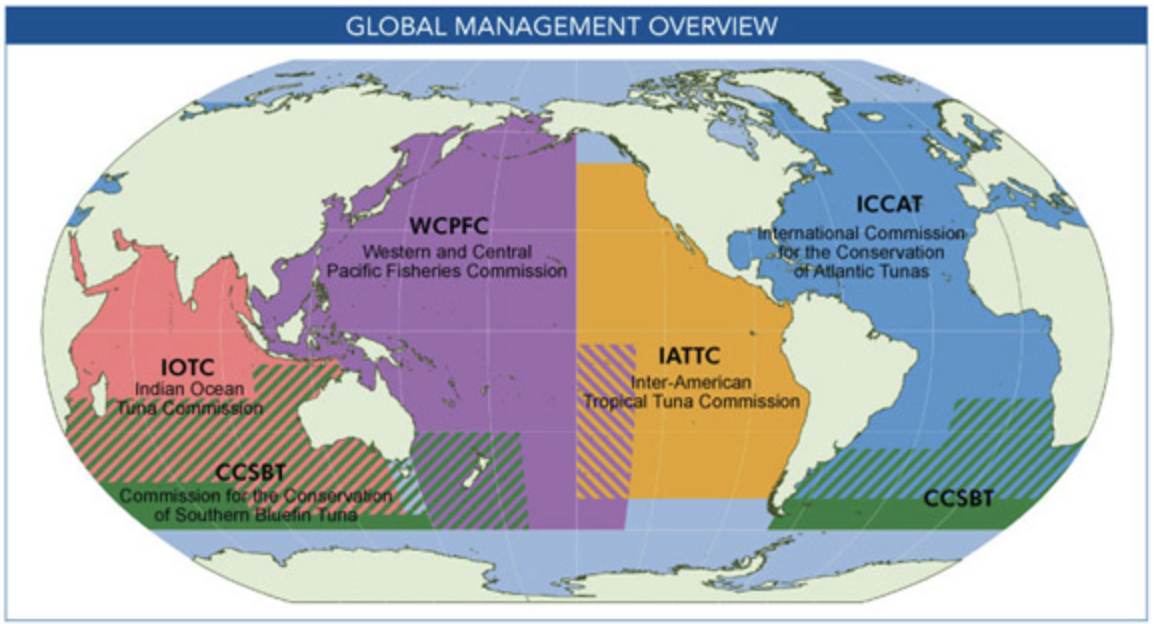
\includegraphics[keepaspectratio]{images/tuna_rfmos.png}}

}

\caption{\label{fig-tuna-rfmos}Global overview of tuna managing Regional
Fisheries Management Organizations.}

\end{figure}%

For the purposes of this paper, we will be scoping the analysis to the
RFMO responsible for the Western Pacific, the \textbf{Western and
Central Pacific Fisheries Commission (WCPFC)}. In order for vessels to
fish for highly migratory species of fish (i.e.~all types of tuna,
marlin, etc.) in the Western and Central Pacific, they must be
registered with WCPFC and follow their regulations. The WCPFC Convention
Area covers over 12 million square nautical miles, or 20\% of the
Earth's oceans (Figure~\ref{fig-wcpfc-ca}).

\begin{figure}

\centering{

\pandocbounded{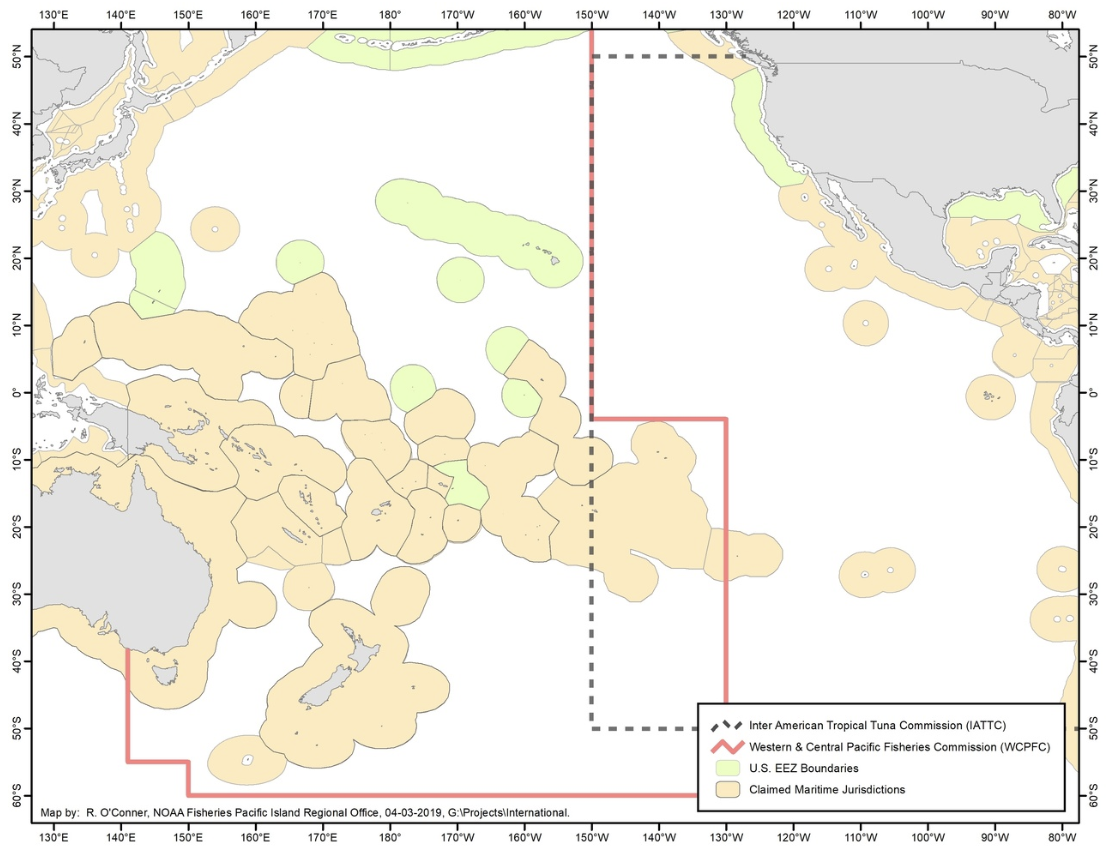
\includegraphics[keepaspectratio]{images/wcpfc_ca.png}}

}

\caption{\label{fig-wcpfc-ca}The WCPFC Convention Area spans the Pacific
Ocean from roughly 141°E to 150°W.}

\end{figure}%

There are currently over 3,000 vessels registered under the WCPFC, with
the most prominent flag states\footnote{Flag State, or Flag State
  Jurisdiction, is defined as: ``A State may exercise jurisdiction over
  a vessel that is registered with the State and flying its flag. This
  exercise of jurisdiction is based on the internationally recognized
  principle that a State may regulate the conduct of its nationals even
  when those nationals are acting outside of the State's
  territory.''(\citeproc{ref-noaa_jurisdiction_vessels}{National Oceanic
  and Atmospheric Administration 2024})} of China, Japan, Chinese Taipei
(Taiwan), and the Philippines.(\citeproc{ref-wcpfc_rfv}{{``WCPFC RFV''}
n.d.}) The WCPFC regulates when, where, what, and how these vessels are
allowed to fish, but only on the High Seas outside any other country's
Exclusive Economic Zone (EEZ)\footnote{Exclusive Economic Zone (EEZ):
  ``A coastal State has sovereign rights to the management of natural
  resources and other economic activities within its EEZ. It does not
  have sovereignty within its EEZ, so foreign vessels possess the same
  non-economic rights within a State's EEZ as on the high seas.''
  (\citeproc{ref-noaa_jurisdiction_vessels}{National Oceanic and
  Atmospheric Administration 2024}) The EEZ extends from the country's
  baseline to 200NM (or when meeting another country's EEZ).}. In order
for a vessel to be registered with WCPFC, they must also be
flagged\footnote{Flag State, or Flag State Jurisdiction, is defined as:
  ``A State may exercise jurisdiction over a vessel that is registered
  with the State and flying its flag. This exercise of jurisdiction is
  based on the internationally recognized principle that a State may
  regulate the conduct of its nationals even when those nationals are
  acting outside of the State's
  territory.''(\citeproc{ref-noaa_jurisdiction_vessels}{National Oceanic
  and Atmospheric Administration 2024})} in a country at that is a
member of the WCPFC\footnote{WCPFC Commission Members: Members -
  Australia, China, Canada, Cook Islands, European Union, Federated
  States of Micronesia, Fiji, France, Indonesia, Japan, Kiribati,
  Republic of Korea, Republic of Marshall Islands, Nauru, New Zealand,
  Niue, Palau, Papua New Guinea, Philippines, Samoa, Solomon Islands,
  Chinese Taipei, Tonga, Tuvalu, United States of America, Vanuatu.
  Participating Territories - American Samoa, Commonwealth of the
  Northern Mariana Islands, French Polynesia, Guam, New Caledonia,
  Tokelau, Wallis and Futuna. Cooperating Non-member(s) - The Bahamas,
  Curacao, Ecuador, El Salvador, Liberia, Panama, Thailand, Vietnam.}.

With 26 member states and over 3,000 vessels, along with large of number
of owners, operators, and corporations, the web of associations within
the fisheries sector for just this RFMO is vast.

\textbf{\emph{Struggling on how to bring it back}}

Using publicly available data on ship registration and associated
information, we hope to examine the files for relationships that might
flag potential concerns or insight into the fishing practices of this
area of the globe.

\subsection{Previous Work}\label{previous-work}

Much previous research has used network analysis to examine fishing
practices. Given the highly complex and layered relationships that can
occur between different entities or information (e.g.~in Dell'Apa et al.
(\citeproc{ref-dellapa_international_2013}{2013}) the authors used SNA
to analyze trade flows of spiny dogfish, revealing how global trade
relationships impact regional conservation outcomes and suggesting that
trade regulations could promote sustainability) that otherwise would be
extremely hard to model simultaneously and understand.

Network analsis can be used to relate information like `vehicle' (in
this case, ship), such as the 2018 paper Ford, Bergseth, and Wilcox
(\citeproc{ref-ford_chasing_2018}{2018}) where the authors utilized
Social Network Analysis (SNA) to identify key ships within the fishing
industry in the Indian Ocean. The researchers utilized AIS data to infer
relationships for vessel who operated in close proximity and found that
Reefer (Refrigerated Cargo Vessels) and Bunkering (Fuel Resupply Ships)
play a key role in the vessel network as identified by their eigenvector
centrality. Another paper Mulvaney et al.
(\citeproc{ref-mulvaney_casting_2015}{2015}) utilized survey data to
establish connections between players in the Great Lake's local
fisheries network. The paper discussed heavily their methodology
constraints with the survey, but also concluded that the fisheries
network included many informal and formal relationships, with the
informal relationships forming a significant portion of the edges.

Again and again, the layered relationship between complex variables in
the oceanic and fishery world shows that different forms of these tools
are highly effecitve. Varlamis et al.
(\citeproc{ref-varlamis_building_2021}{2021}) go through an interesting
deep dive on the utilization of AIS to create vessel traffic networks.
While this paper may not ultimately be helpful for overfishing, these
types of visualization and aggregation of data in a relationship format
that can be analyzed is incredibly powerful.

Similarly in terms of applications that may not have merit in this
initial data study, Marín and Berkes
(\citeproc{ref-marin_network_2010}{2010}) examined co-management
networks in Chilean small-scale fisheries, finding that power was highly
centralized in government institutions, with limited cooperation among
fisher associations, and recommending policy changes for more
participatory governance - something that is far beyond classic data
analysis and using qualitative data to reveal relationships.

The qualtitative element is important to remember for future work post
quantitaive analysis, e.g.~for intervation - Dell'Apa et al.
(\citeproc{ref-dellapa2014dogfish}{2014}) expanded on previous work to
explore how stakeholder networks influence fishery management policies
for spiny dogfish, showing the importance of network structures in
shaping effective governance.

These interventions can help us to not just implement policy, but to
`live-manage' its implementation in such a complex ecosystem.

A critical component of Nogueira et al.
(\citeproc{ref-nogueira2023dynamics}{2023}) analysis of fisheries in the
Azores was converting time-series catch data into network structures.
Their time sensitive identification of key species associations and
critical fishing nodes relevant for sustainable management strategies
show extreme promise not just for analysis and results, but for
recommendations and a far more effective way to achieve our goal; which
is to ultimately sustain healthy fish populations and protein sources
for the future inhabitants of the planet.

The previous work of many authors, Nogueira et al.
(\citeproc{ref-nogueira_dynamics_2025}{2025}) included, is applying
complex network analysis and metrics to fisheries data - whether in
Nogueira et al. (\citeproc{ref-nogueira_dynamics_2025}{2025}) from the
Azores Islands, which focused on uncovering structural patterns in the
ecosystem and offering insights for sustainable policy and marine
resource management, or whether in the social dynamics that can help
facilitate a different form of management.

\section{Data Source}\label{data-source}

WCPFC Registry of Fishing Vessels (RFV)

\phantomsection\label{refs}
\begin{CSLReferences}{1}{0}
\bibitem[\citeproctext]{ref-global_fish_watch_2024}
{``Commercial Fishing. Global Fishing Watch.''} 2024. October 24, 2024.
\url{https://globalfishingwatch.org/commercial-fishing/}.

\bibitem[\citeproctext]{ref-dellapa_international_2013}
Dell'Apa, Andrea, Jeffrey C. Johnson, David G. Kimmel, and Roger A.
Rulifson. 2013. {``The International Trade and Fishery Management of
Spiny Dogfish: A Social Network Approach.''} \emph{Ocean \& Coastal
Management} 80 (August): 65--72.
\url{https://doi.org/10.1016/j.ocecoaman.2013.04.007}.

\bibitem[\citeproctext]{ref-dellapa2014dogfish}
---------. 2014. {``The International Trade and Fishery Management of
Spiny Dogfish: A Social Network Approach.''} \emph{Ocean \& Coastal
Management} 96: 165--72.
\url{https://doi.org/10.1016/j.ocecoaman.2014.05.007}.

\bibitem[\citeproctext]{ref-ford_chasing_2018}
Ford, Jessica H., Brock Bergseth, and Chris Wilcox. 2018. {``Chasing the
Fish Oil---Do Bunker Vessels Hold the Key to Fisheries Crime
Networks?''} \emph{Frontiers in Marine Science} 5 (August).
\url{https://doi.org/10.3389/fmars.2018.00267}.

\bibitem[\citeproctext]{ref-marin_network_2010}
Marín, Andrés, and Fikret Berkes. 2010. {``Network Approach for
Understanding Small-Scale Fisheries Governance: The Case of the Chilean
Coastal Co-Management System.''} \emph{Marine Policy} 34 (5): 851--58.
\url{https://doi.org/10.1016/j.marpol.2010.01.007}.

\bibitem[\citeproctext]{ref-mulvaney_casting_2015}
Mulvaney, Kate K., Seungyoon Lee, Tomas O. Höök, and Linda S. Prokopy.
2015. {``Casting a Net to Better Understand Fisheries Management: An
Affiliation Network Analysis of the Great Lakes Fishery Commission.''}
\emph{Marine Policy} 57 (July): 120--31.
\url{https://doi.org/10.1016/j.marpol.2015.03.008}.

\bibitem[\citeproctext]{ref-noaa_jurisdiction_vessels}
National Oceanic and Atmospheric Administration. 2024. {``Jurisdiction
over Vessels.''} \url{https://www.noaa.gov/jurisdiction-over-vessels}.

\bibitem[\citeproctext]{ref-nogueira2023dynamics}
Nogueira, Brenda, Ana Torres, Nuno Moniz, and Gui M. Menezes. 2023.
{``Dynamics of Fisheries in the Azores Islands: A Network Analysis
Approach.''} \url{https://arxiv.org/abs/2309.09378}.

\bibitem[\citeproctext]{ref-nogueira_dynamics_2025}
---------. 2025. {``Dynamics of~Fisheries in~the~Azores Islands: A
Network Analysis Approach.''} In \emph{Progress in Artificial
Intelligence}, edited by Manuel Filipe Santos, José Machado, Paulo
Novais, Paulo Cortez, and Pedro Miguel Moreira, 297--308. Cham: Springer
Nature Switzerland. \url{https://doi.org/10.1007/978-3-031-73500-4_25}.

\bibitem[\citeproctext]{ref-poortvliet_sustainable_2024}
Poortvliet, Dave. 2024. {``Sustainable Fisheries Management Begins with
Vessel Tracking. Global Fishing Watch.''} October 24, 2024.
\url{https://globalfishingwatch.org/fact-sheet/sustainable-fisheries-management-begins-with-vessel-tracking/}.

\bibitem[\citeproctext]{ref-varlamis_building_2021}
Varlamis, Iraklis, Ioannis Kontopoulos, Konstantinos Tserpes, Mohammad
Etemad, Amilcar Soares, and Stan Matwin. 2021. {``Building Navigation
Networks from Multi-Vessel Trajectory Data.''} \emph{{GeoInformatica}}
25 (1): 69--97. \url{https://doi.org/10.1007/s10707-020-00421-y}.

\bibitem[\citeproctext]{ref-wcpfc_rfv}
{``WCPFC RFV.''} n.d. Accessed April 23, 2025.
\url{https://vessels.wcpfc.int/statistics/by-vessel-type}.

\bibitem[\citeproctext]{ref-pew_faq_2012}
{``What Is a Regional Fishery Management Organization. Pew.''} 2012.
February 23, 2012. \url{http://bit.ly/102wBKa}.

\end{CSLReferences}




\end{document}
